\documentclass{scrartcl}

\usepackage[ngerman]{babel}
\usepackage[T1]{fontenc}
\usepackage[utf8]{inputenc}
\usepackage{graphicx, caption}
\graphicspath{ {./img/} }
\usepackage{amsmath}
\newcommand{\Mod}[1]{\ (\mathrm{mod}\ #1)}
\usepackage[parfill]{parskip}
\usepackage{siunitx}
\usepackage[section]{placeins}


\begin{document}
    \begin{titlepage}
        \title{Computergrafik 1 - Beleg}
        \subtitle{Dokumentation}
        \author{Theresa Schüttig}
        \maketitle
    \end{titlepage}

    \tableofcontents
    \newpage

    \section{Aufgabenbeschreibung}

        Schreiben Sie ein Programm in C/C++, das unter Verwendung von OpenGL, Vertex- und
        Fragment-Shadern folgende Aufgaben realisiert. \newline


        \textbf{Aufgabe 1} \\
        Geometrische Objekte: Erzeugen Sie eine interaktive zeitlich animierte Szene mit mehreren
        unterschiedlichen farblichen und texturierten dreidimensionalen geometrischen Objekten. \newline

        \textbf{Aufgabe 2} \\
        Beleuchtung: Beleuchten Sie die Szene mit verschiedenartigen Lichtquellen so, dass auf den
        Objekten unterschiedliche Beleuchtungseffekte sichtbar werden. \\

        \textbf{Aufgabe 3}
        Ansicht: Stellen Sie die Szene gleichzeitig in verschiedenen Ansichten und Projektionen in
        mehreren Viewports des Anzeigefensters dar. \\

        \textbf{Aufgabe 4} \\
        Programm: Stellen Sie das komplette Programm in Quelltextform als Visual-Studio-C++-
        Projekt und in ausführbarer Form als exe-File derart bereit, dass die Lauffähigkeit auf den
        Computern des Praktikumslabors der Lehrveranstaltung gewährleistet ist. \\

        \textbf{Aufgabe 5} \\
        Dokumentation: Fertigen Sie eine Systemdokumentation in Form eines pdf-Dokumentes von
        etwa 10 Seiten an, die Deckblatt, Gliederung, Aufgabenbeschreibung, Lösungsansatz,
        Lösungsumsetzung, Installations- und Bedienungsanleitung, einige Bildschirm-Snapshots,
        Probleme, Ergebnisse, Literatur- und Quellenverzeichnis enthält. \\

        \textbf{Aufgabe 6} \\
        Abgabe: Demonstrieren Sie die Ergebnisse der Aufgaben 4 und 5 an einem Computer des
        Praktikumslabors der Lehrveranstaltung und übergeben Sie diese in einem Verzeichnis
        „Name\_Vorname\_Bibliotheksnummer“. \\

        \textbf{Zeitplan} \\
        Die Ausgabe der Aufgabenstellung erfolgt zu Beginn der Lehrveranstaltungszeit. Die Abgabe
        der Ergebnisse erfolgt spätestens zum Ende der Lehrveranstaltungszeit. \\

    \section{Lösungsansatz}
        \subsection{Vorüberlegung}
            Das Programm soll 4 Kegel darstellen, die sich mit gleicher Geschwindigkeit 
            und in gleicher Richtung auf einer Kreisbahn bewegen, auf der sie gleichmäßig 
            verteilt sind. Der Radius der Kreisbahn schwankt in Abhängigkeit der Zeit 
            gleichmäßig um einen festen Wert. Die Spitze der Kegel soll dabei stets auf 
            den Mittelpunkt des Kreises gerichtet sein. Zwei der Kegel besitzen eine 
            Holztextur, die anderen zwei Kegel besitzen eine Metalltextur und glänzen 
            zusätzlich. Kegel aus dem gleichen Material befinden sich auf der Kreisbahn 
            gegenüber. \\
            Die Szene wird durch ein Richtungslicht und 4 verschiedenfarbige Punktlichte, 
            welche als einfarbige Würfel ohne Schattierung dargestellt werden, beleuchtet. 
            Jeder Würfel bewegt sich auf einer eigenen Kreisbahn mit festem Radius, die 
            einen Punkt enthält, der Mittelpunkt der Kreisbahn der Kegel ist. Der Abstand
            zwischen dem Mittelpunkt einer Lichtkreisbahn und dem Mittelpunkt der Kegelkreisbahn
            ist bei jeder Lichtquelle gleich. Die Ebene, 
            auf der die Kreisbahn einer Lichtquelle liegt und die Ebene der Kreisbahn, 
            auf der die Kegel liegen, sind orthogonal zueinander. Die Schnittpunkte 
            zwischen der Ebene einer Lichtkreisbahn und der Kegelkreisbahn sind 
            gleichmäßig auf der Kegelkreisbahn verteilt. Alle Würfel befinden sich 
            entweder über oder unter (abhängig vom Blickwinkel) der Ebene der 
            Kegelkreisbahn, wenn sie sich auf dessen Mittelpunkt zubewegen. 
            Die Lichtquellen sollen nacheinander mit gleichem Zeitabstand auf 
            diesen Mittelpunkt treffen. \\
            Die Bewegung aller Objekte erfolgt periodisch und die Größe der Kreisbahnen 
            und Objekte sind so zu wählen, dass zu keinem Zeitpunkt zu einer Überlappung 
            zwischen zwei Objekten kommt. \\
            Im Fenster sollen vier verschiedene Viewports enthalten sein, von denen jeder 
            die Szene aus einem anderen Blickwinkel darstellt. Für einen Viewport kommt
            eine orthographische Projektion zum Einsatz, für alle anderen Viewports wird eine perspektivische Projektion verwendet.
            Zudem kann der Nutzer in einem der Viewports zoomen und die Szene rotieren.
        \newpage
        \subsection{Skizze}
            \begin{figure}[!htb]
            \centering
            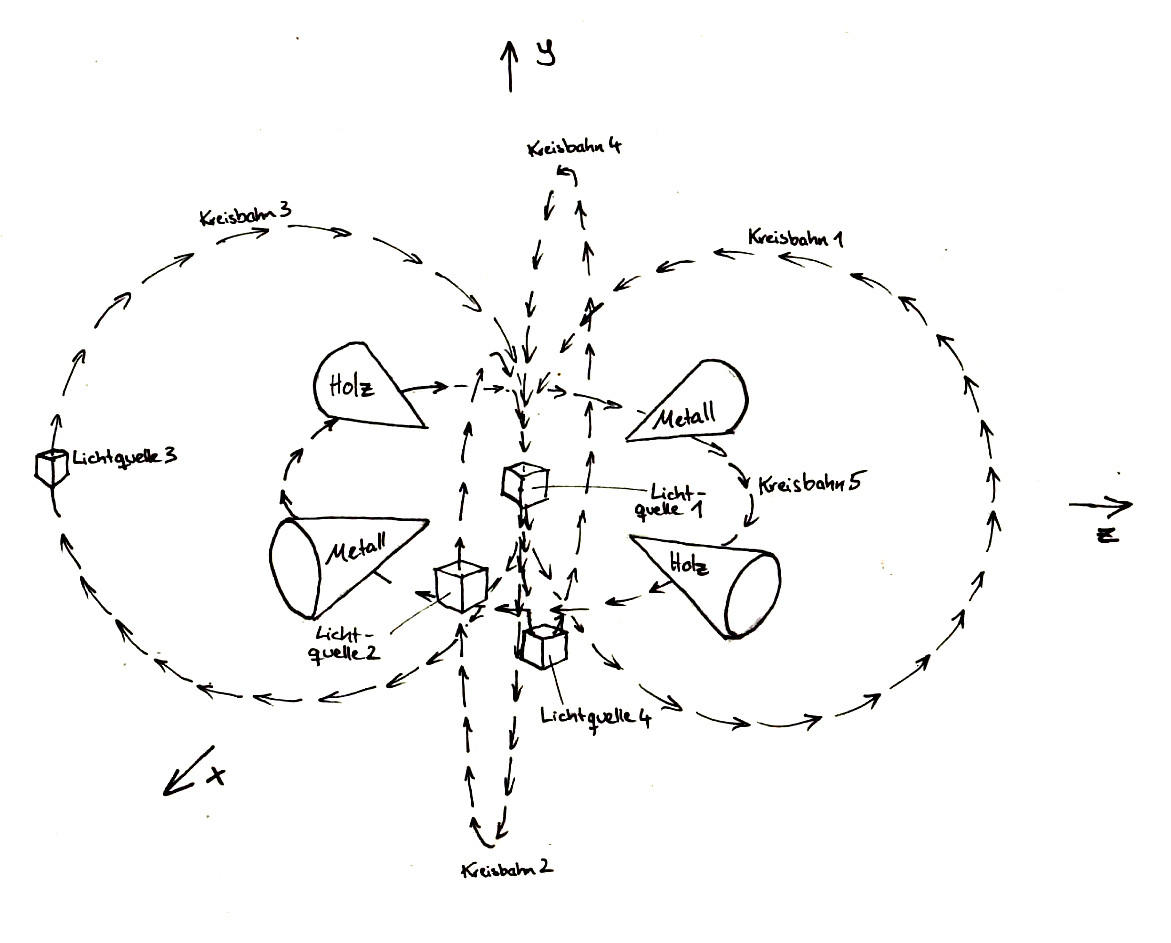
\includegraphics{skizze.jpeg}
        \end{figure}
        \newpage

    \section{Lösungsumsetzung}
    %t.b.d.
        \subsection{Berechnungen}
            Die Kegel rotieren um den Koordinatenursprung und besitzen folgende Koordinaten: \par
            Kegel 1: $K_{1}$(a | 0 | -b) \\
            Kegel 2: $K_{2}$(b | 0 | a) \\
            Kegel 3: $K_{3}$(-a | 0 | b) \\
            Kegel 4: $K_{4}$(-b | 0 | a) \\
             
            a und b werden folgendermaßen berechnet:
            \begin{center}
            $a = sin(f(t))\cdot (1,025-0,35\cdot sin(2\cdot f(t)))$ \\
            $b = cos(f(t))\cdot (1,025-0,35\cdot sin(2\cdot f(t)))$ \\
            \end{center}
            f(t) ist eine von der Zeit abhängige Funktion, die den aktuellen Winkel im Gradmaß angibt und folgendermaßen definiert ist:
            \begin{center}
            $f:[0, \infty)\rightarrow [0,359]$, $t\mapsto t\cdot 10^{-2} \mod 360$ 
            \end{center}

            Der Radius schwankt also periodisch zwischen $0,675$LE und $1,375$LE mit einer Periodendauer von 1,8s, wobei der Radius als Abstand zwischen dem Koordinatenursprung und dem Mittelpunkt eines Kegels definiert ist.
            Für die Höhe eines Kegels wurde 1LE festgelegt, so dass auf der x-z-Ebene ein Kreis mit Radius r = 0,175LE entsteht, durch den laut Satz des Pythagoras in jedem Fall ein Würfel mit einer Kantenlänge von bis zu
            $\sqrt{2\cdot r^2}$ = 0,247LE über den Mittelpunkt der Kegelkreisbahn gelenkt werden kann, ohne dass es zur Überlappung mit einem Kegel kommt. Im Programm wurden für die Kantenlänge 0,25LE festgelegt.
            Da sich im Mittelpunkt der Kegelkreisbahn kein Würfel befindet, wenn die Kegelkreisbahn ihren minimalen Radius erreicht, kommt es mit diesem leicht höheren Wert zu keiner Überlappung.\\
            Damit die Kegelspitzen in Richtung Koordinatenursprung zeigen, muss jeder Kegel um einen Vektor rotiert werden, der die Kegelmitte schneidet und parallel zur y-Achse verläuft.
            Der Winkel $\alpha_i$, um den der Kegel i gedreht werden muss, wird folgendermaßen berechnet: \\
            $\alpha_i = -f(t) + (i-1)\cdot \ang{90}$ \\
            
            Die Lichtquellen rotieren um folgende Koordinaten: \\
            Licht 1: A(1,5 | 0 | 0) \\
            Licht 2: B(0 | 0 | -1,5) \\
            Licht 3: C(-1,5 | 0 | 0) \\
            Licht 4: D(0 | 0 | 1,5) \\

            Auf Basis der Angaben im Lösungsansatz lassen sich die von der Zeit abhängigen Koordinaten $L_{i}$, $i\in \{1,2,3,4\}$ der Lichter 1$-$4 folgendermaßen berechnen: \par
            $L_{1} = A +   \begin{pmatrix}
                            -sin(f(t))\cdot 1,5 \\
                            cos(f(t))\cdot 1,5 \\
                            0
                        \end{pmatrix}$ \par
            $L_{2} = B +   \begin{pmatrix}
                            0 \\
                            cos(f(t)+\ang{90})\cdot 1,5 \\
                            sin(f(t)+\ang{90})\cdot 1,5 
                        \end{pmatrix}$ \par
            $L_{3} = C +   \begin{pmatrix}
                            sin(f(t)+\ang{180})\cdot 1,5 \\
                            cos(f(t)+\ang{180})\cdot 1,5 \\
                            0
                        \end{pmatrix}$ \par
            $L_{4} = D +   \begin{pmatrix}
                            0 \\
                            cos(f(t)+\ang{270})\cdot 1,5 \\
                            -sin(f(t)+\ang{270})\cdot 1,5
                        \end{pmatrix}$ \\

        \subsection{Programmstruktur}
            \subsubsection*{Main.cpp}
                \begin{itemize}
                    \item \textbf{void main(int argc, char *argv[])}
                    Nimmt notwendige Initialiserungen zur Nutzung von OpenGL vor, 
                    erzeugt ein Fenster und legt bestimmte in \textit{Program.cpp} definierte 
                    Funktionen als Callback-Funktionen fest.
                \end{itemize}

            \subsubsection*{Program.cpp}
                \begin{itemize}
                \item \textbf{void init()}
                    Generiert Texturen und VAOs, VBOs und Puffer, ermittelt die Positionen 
                    der Shader-Variablen, übergibt dem Fragment-Shader die Lichtfarben und 
                    aktiviert die Tiefenprüfung.
                \item \textbf{void display()}
                    Leert den Farb- und Tiefenpuffer, befüllt diesen neu und erzeugt vier 
                    quadratische Viewports gleicher Größe. Vor dem Rendern eines Viewports 
                    werden die Matrizen \textit{View} und \textit{Projection} modifiziert.
                \item \textbf{void renderScene()}
                    Berechnet einen von der Zeit abhängigen Winkel, der im Schnitt alle 10ms 
                    um \ang{1} erhöht wird. Über diesen Winkel werden die Kegel- und Würfelpositionen
                    berechnet. Für jedes Objekt werden die Matrizen \textit{Model} und
                    \textit{ModelViewProjection} und \textit{NormalMatrix} berechnet. 
                    Vor dem Rendern der Würfel wird dem Fragment-Shader die Nummer der 
                    jeweiligen Lichtquelle über das Setzen von \textit{isLightSource} übergeben. 
                    Nach dem Rendern wird diese Variable wieder auf 0 gestetzt. 
                \item \textbf{void loadTextures()}
                    Bindet die Texturen, deren Pfade in \textit{texturePaths} gespeichert sind, an 
                    \textit{GL\_TEXTURE\_2D}.
                \item \textbf{void setViewPoint()}
                    Berechnet die Matrix \textit{View} basierend auf der vom Nutzer festgelegten 
                    Betrachterposition und übergibt dem Fragment-Shader die Betrachterposition.
                \item \textbf{void reshape(int w, int h)}
                    Aktualisiert die Variablen \textit{width} und \textit{height} für die Fenstergröße, 
                    wenn diese geändert wird.
                \item \textbf{void timer(int value)}
                    Wird kontinuierlich nach minimal 10ms erneut aufgerufen und leitet den erneuten Aufruf von display ein.
                \item \textbf{void keyboard(unsigned char theKey, int mouseX, int mouseY)}
                    Wird bei Betätigen einer Taste der Tastatur aufgerufen und verändert die 
                    Variablen, die Entfernung der Blickposition vom Mittelpunkt der Szene bestimmen.
                \item \textbf{void special(int specKey, int mouseX, int mouseY)}
                    Wird aufgerufen, wenn eine Funktions- oder Pfeiltaste betätigt wird. Wurde 
                    eine Pfeiltaste betätigt, so verändert die Funktion Variablen, die die 
                    Blickposition bestimmen.
                \item \textbf{void motion(int mouseX, int mouseY)}
                    Wird bei Mausbewegung aufgerufen, wenn mindestens eine Maustaste gedrückt 
                    gehalten wird und verändert Variablen, die die Blickposition bestimmen.
                \end{itemize}

            \subsubsection*{Data.hpp}
                Enthält die Bezeichner für die VAOs, VBOs und Buffer-Objekte, welche in 
                \textit{Cone.cpp}, \textit{Cube.cpp} und \textit{Program.cpp} verwendet 
                werden.
            \subsubsection*{Cube.cpp}
                \begin{itemize}
                    \item \textbf{void generateCube()}
                        Erzeugt die Würfel- und Texturkoordinaten sowie Normalenvektoren, 
                        bindet diese an den \textit{GL\_ARRAY\_BUFFER} und aktiviert die Attributarrays 
                        für den Vertex-Shader.
                    \item \textbf{void drawCube(int texID)}
                        Rendert einen Würfel mit der Textur, der \textit{texID} als Bezeichner zugewiesen wurde.
                \end{itemize}
            \subsubsection*{Cone.cpp}
                \begin{itemize}
                    \item \textbf{void generateCone()}
                        Erzeugt die Kegel- und Texturkoordinaten sowie Normalenvektoren, bindet diese an 
                        den \textit{GL\_ARRAY\_BUFFER} und aktiviert die Attributarrays für den Vertex-Shader.
                    \item \textbf{void drawCone(int texID)}
                        Rendert einen Kegel mit der Textur, der \textit{texID} als Bezeichner zugewiesen wurde.
                    \item \textbf{void calcConeTexCoords(float h, float r, float vertices[][2])}
                        Berechnet die Texturkoordinaten für einen Kegel mit der Höhe \textit{h} und dem Radius 
                        \textit{r} und speichert diese im Array \textit{vertices}, welches mindestens eine Größe von 
                        $12 \cdot$ \textit{NumVertices} besitzen muss.
                \end{itemize}
            \subsubsection*{LoadShader.cpp}
                \begin{itemize}
                \item \textbf{GLuint LoadShaders(const char *vertexFilePath, const char *fragmentFilePath)}
                    Kompiliert den Vertex- und Fragment-Shader, deren Pfade als Parameter übergeben werden.
                \end{itemize}
            \subsubsection*{main.vs}
                \begin{itemize}
                \item \textbf{void main()}
                    Berechnet \textit{gl\_Position} und übergibt dem Fragment-Shader den Normalenvektor 
                    und Textur- und Vertexkoordinaten.
                \end{itemize}
            \subsubsection*{main.fs}
                \begin{itemize}
                \item \textbf{void main()}
                    Summiert die Lichter aller Lichtquellen, und legt das Ergebnis als 
                    Farbe des Fragments fest, falls \textit{isLightSource} 0 ist. 
                    Andernfalls erhält das Fragment eine leicht aufgehellte Variante der Farbe 
                    der Lichtquelle.
                \item \textbf{vec3 calcLight(int lightID)}
                    Berechnet den ambienten, diffusen und spekularen Anteil der Lichtquelle mit der 
                    Bezeichnung \textit{lightID}. Ist \textit{useSpecularLight} 0, so wird der spekulare Anteil 
                    auf 0 gesetzt. Ist \textit{lightID} 4, so wird \textit{lightDir} als Richtungsvektor 
                    des Lichts verwendet, andernfalls wird dieser über die Lichtposition (\textit{lightPos[lightID]}) 
                    und die Fragmentposition (\textit{FragPos}) ermittelt. Zurückgegeben wird das Produkt aus der 
                    Texturfarbe und der Summe des ambienten, diffusen und spekularen Anteils.
                \end{itemize}
    \newpage
    \section{Installation}
        Unabhängig vom Betriebssystem müssen vor der Installation die Bibliotheken 
        \textit{OpenGL}, \textit{GLUT}, \textit{GLM} und \textit{FreeImage} installiert 
        werden. Die ausführbare Datei befindet sich nach der Installation im Verzeichnis 
        \textit{bin}.
        \subsection{Windows} %t.b.d.
            Unter Windows kann die Projektionmappendatei mit Visual Studio Community 
            geöffnet und über Erstellen -> Projektmappe kompiliert werden.
      %  \subsection{Linux}
      %      Unter Linux kann das Programm über das Kommando \textit{make} installiert 
      %      werden. Der Nutzer muss sich dafür im Verzeichnis \textit{src} befinden.

    \section{Bedienung}
        \subsection{Entfernen und Wiederhinzufügen von Lichtquellen}
            Jedes Punktlicht kann durch das Betätigen einer bestimmten Taste entfernt 
            oder wieder hinzugefügt werden. Für jede Lichtquelle kann dieser Vorgang 
            beliebig oft wiederholt werden. \par
        \begin{tabular}{| l | l |}
            \hline
            Taste & Farbe der Lichtquelle \\ \hline
            R & rot \\ \hline
            O & orange \\ \hline
            G & gelb \\ \hline
            B & blau \\ \hline
        \end{tabular}

        \subsection{Rotieren und Zoomen}
            Im linken oberen Viewport kann der Nutzer in der Szene zoomen und rotieren. Das Zooming 
            erfolgt über die Pfeiltasten oder über das Gedrückthalten einer Maustaste mit 
            gleichzeitigem Bewegen der Maus. In Richtung Mittelpunkt kann über die V-Taste 
            gezoomt werden, das Herauszoomen erfolgt über die Z-Taste.

        \subsection{Beenden des Programms}
            Das Programm kann über das Schließen des Fensters oder das Betätigen der 
            E-Taste beendet werden.
    \newpage
    \section{Screenshots}

        \begin{figure}[!htpb]
            \centering
            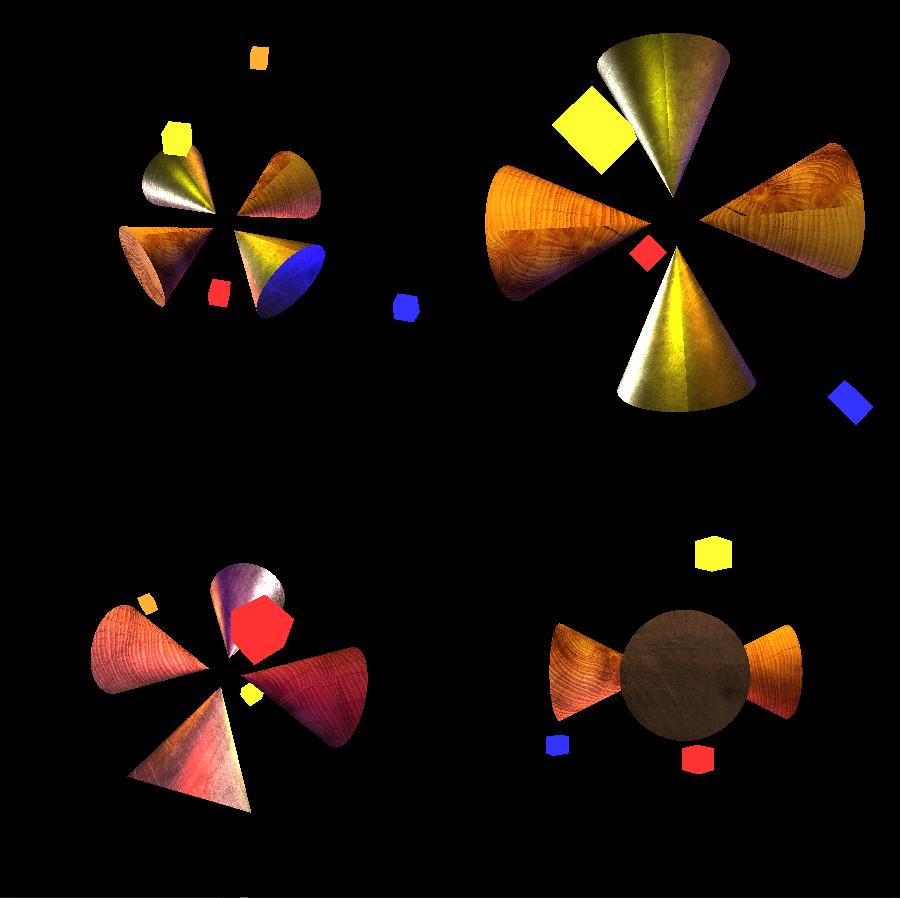
\includegraphics[scale=0.25]{scrshot2.jpg}
            \caption*{Alle Viewports mit allen Lichtquellen}
        \end{figure}
        \begin{figure}[!htpb]
            \centering
            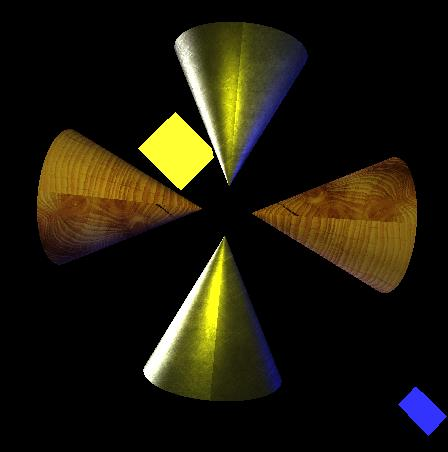
\includegraphics[scale=0.5]{scrshot3.jpg}
            \caption*{Rechter unterer Viewport ohne rotes und oranges Punktlicht}
        \end{figure}
        \begin{figure}[!htpb]
            \centering
            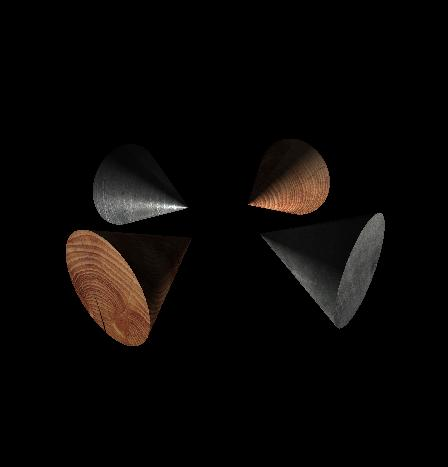
\includegraphics[scale=0.5]{scrshot1.jpg}
            \caption*{Linker oberer Viewport ohne Punktlichter}
        \end{figure}
    \newpage

    \section{Probleme}
        \subsection{Keine nahtlose Texturierung}
            Auf der Mantelfläche und zwischen Mantel- und Grundfläche befinden sich 
            Nahtstellen. Diese könnte man entfernen, indem man unter Verwendung der 
            vom Programm erstellten Texturkoordinaten eine speziell für die Kegel nahtlose 
            Textur erstellt.

        \subsection{Kein Schattenwurf}
            Die in der Szene dargestellten Objekte werfen keinen Schatten auf ein anderes 
            Objekt, wenn sie sich zwischen diesem und einer Lichtquelle befinden, woraus 
            ein Verlust von Realismus folgt. Zur Lösung des Problems bietet sich der 
            Einsatz von Shadow-Mapping an.

        \subsection{Blick in das Innere der Objekte möglich}
        Durch geschicktes Zoomen und Rotieren der Szene kann der Betrachter die 
        Blickposition in das Innere eines Objektes verschieben, was im Idealfall nicht 
        möglich sein sollte.
        Um dies zu verhindern, kann im Hauptprogramm überprüft werden, ob die Position 
        des Betrachters bei einer bestimmten Veränderung mit einem der Objekte kollidieren würde. 
        In diesem Fall würde diese Änderung nicht vorgenommen werden.
    \newpage
    \section{Ergebnisse}
        Die Anfertigung des Belegs half, Kenntnisse von Grundlagen, insbesondere Licht und Texturen, zu festigen und zu verstehen,
        wie mehrere, sich bewegenden Lichtquellen in einer Anwendung implementiert werden können.
    \newpage    

    \section{Literatur- und Quellenverzeichnis}
        \subsection{Literatur}
        \begin{itemize}
            \item OpenGL Programming Guide, Addison Wesley, 2013, 8. Auflage
            \item Vorlesungsskript
            \item https://learnopengl.com/
        \end{itemize}
        \subsection{Quellcode}
        \begin{itemize}
        \item einzelne Funktionen: Praktikumsunterlagen
        \end{itemize}
        \subsection{Bilder}
        \begin{itemize}
        \item Holztextur: https://pixabay.com/photos/wood-tree-spruce-picea-conifer-3212803/
        \item Metalltextur: https://pixabay.com/photos/background-texture-metal-scratches-1172581/
        \end{itemize}


\end{document}